%\documentclass[]{article}
%
%\usepackage{subfig}
%\usepackage[]{graphicx}
%
%\begin{document}
%	\begin{figure}% >>>
%		\centering
%		\begin{minipage}[t]{.45\linewidth}
%			\subfloat[text1]
%			{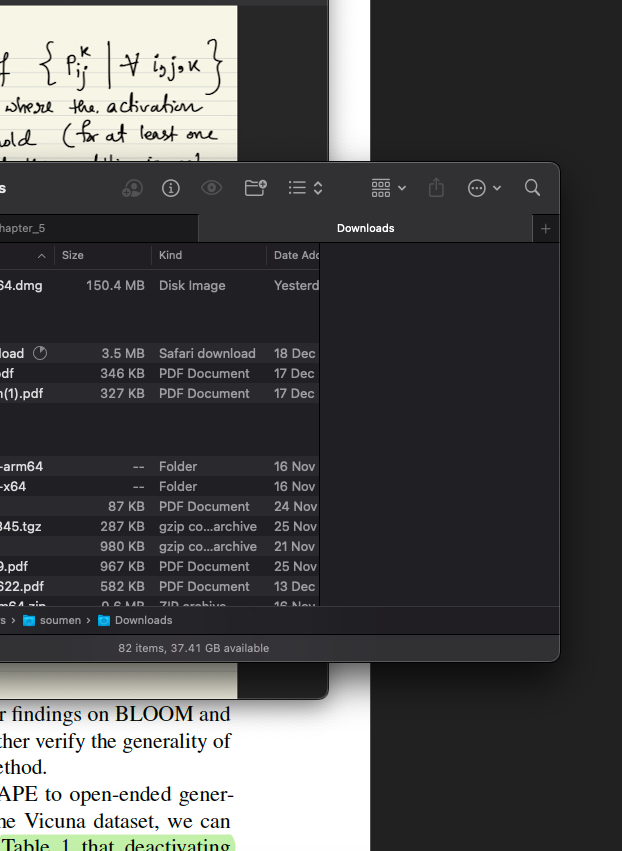
\includegraphics[width=\linewidth]{test.png}}%
%		\end{minipage}%
%		\hfill
%		\begin{minipage}[b]{.45\linewidth}
%			\subfloat[text2]
%			{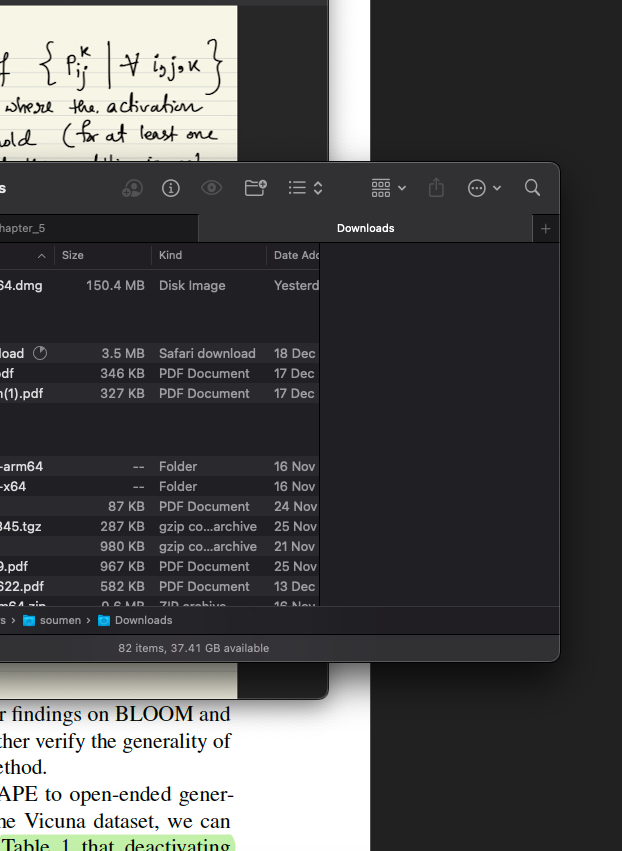
\includegraphics[width=.5\linewidth]{test.png}}\\
%			\subfloat[text3]
%			{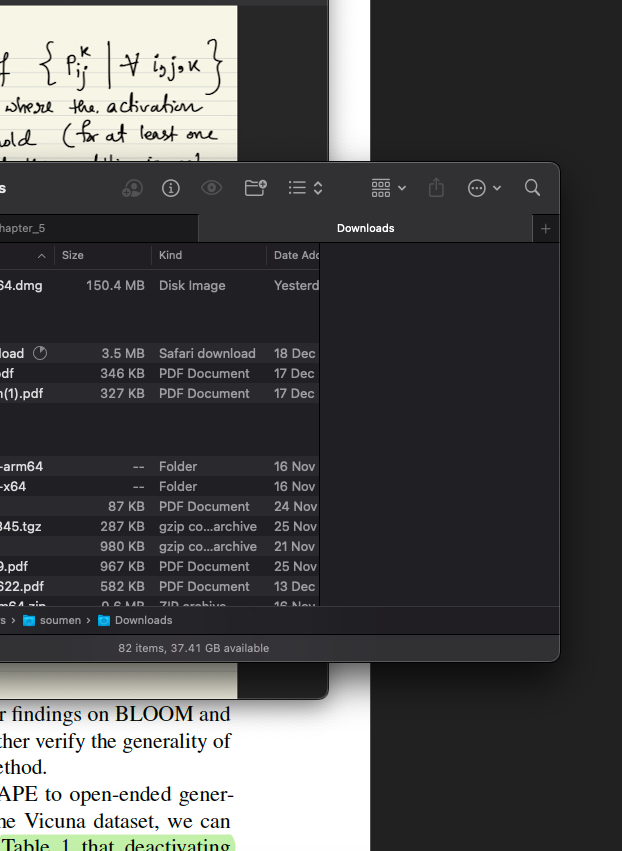
\includegraphics[width=.5\linewidth]{test.png}}%
%		\end{minipage}%
%		\caption
%		{%
%			Caption.%
%			\label{fig:caption}%
%		}%
%	\end{figure}% <<<
%	
%\end{document}

\documentclass[a4paper,12pt]{book}
\usepackage{subcaption}
\usepackage[]{graphicx}

\begin{document}
	\begin{figure}[th]
		\begin{subfigure}[b]{0.1}
			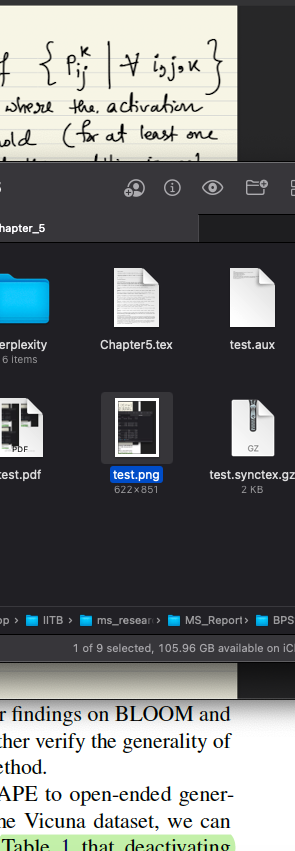
\includegraphics[width=\textwidth]{testb.png}
			\caption{1}
		\end{subfigure}
		\hfill  % NOTE1: hfill moves horizontally stacked objects as far apart as it can
		\begin{subfigure}[b]{0.321}
			\begin{subfigure}[t]{0.1}
				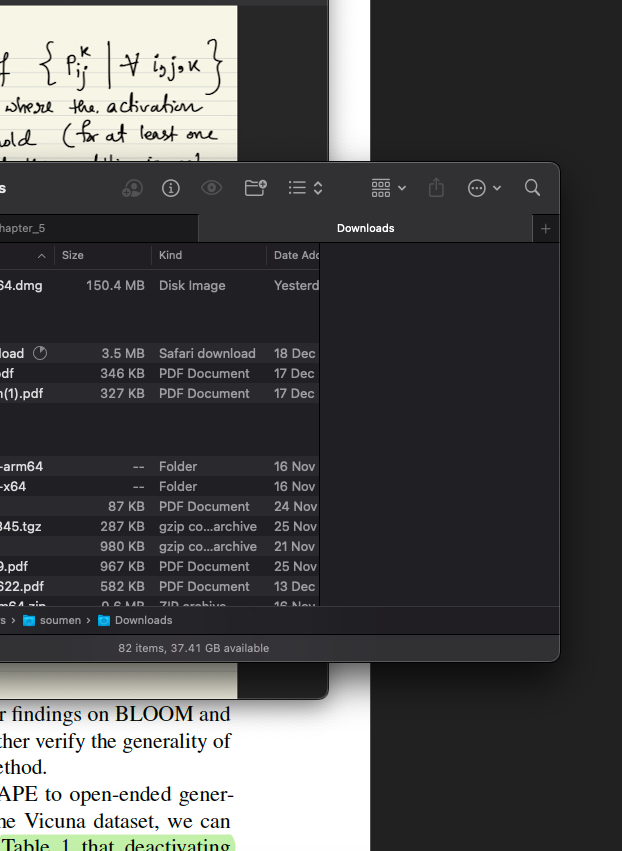
\includegraphics[width=\textwidth]{test.png}
				\caption{2}
			\end{subfigure}
			% NOTE2: two empty lines = 1 linebreak
			
			
			\begin{subfigure}[b]{0.1}
				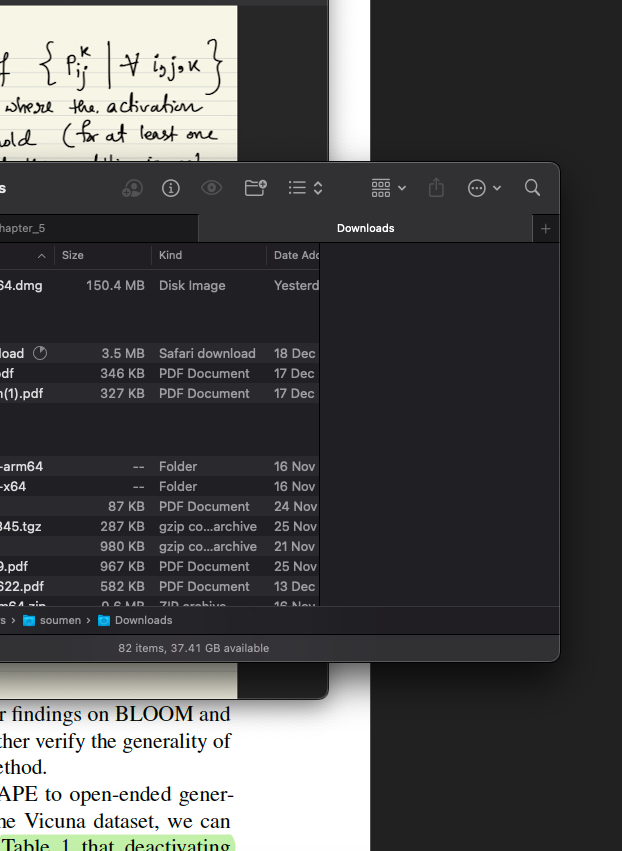
\includegraphics[width=\textwidth]{test.png}
				\caption{3}
			\end{subfigure}
		\end{subfigure}
		
		\caption{figure caption}
	\end{figure}
\end{document}
